%
% File acl2020.tex
%
%% Based on the style files for ACL 2020, which were
%% Based on the style files for ACL 2018, NAACL 2018/19, which were
%% Based on the style files for ACL-2015, with some improvements
%%  taken from the NAACL-2016 style
%% Based on the style files for ACL-2014, which were, in turn,
%% based on ACL-2013, ACL-2012, ACL-2011, ACL-2010, ACL-IJCNLP-2009,
%% EACL-2009, IJCNLP-2008...
%% Based on the style files for EACL 2006 by 
%%e.agirre@ehu.es or Sergi.Balari@uab.es
%% and that of ACL 08 by Joakim Nivre and Noah Smith

\documentclass[11pt,a4paper]{article}

\usepackage{times}
\usepackage{tabularx}
\usepackage{latexsym}
\usepackage{graphicx}
\usepackage[hyperref]{acl2020}
\usepackage{cite}
\usepackage{sans}
\renewcommand{\arraystretch}{1.3}
\renewcommand{\UrlFont}{\ttfamily\small}
\usepackage{biblatex} %Imports biblatex package
\addbibresource{references.bib}
% This is not strictly necessary, and may be commented out,
% but it will improve the layout of the manuscript,
% and will typically save some space.
\usepackage{microtype}

\aclfinalcopy % Uncomment this line for the final submission
%\def\aclpaperid{***} %  Enter the acl Paper ID here

%\setlength\titlebox{5cm}
% You can expand the titlebox if you need extra space
% to show all the authors. Please do not make the titlebox
% smaller than 5cm (the original size); we will check this
% in the camera-ready version and ask you to change it back.

\newcommand\BibTeX{B\textsc{ib}\TeX}

\title{Hierarchical Modeling for Sparse Labeled Data for Accurate Classification}

\author{Gauransh Sawhney \\\And
  Sanjeet Kapadia \\\And Kumar Mallikarjuna\\}

\date{}

\begin{document}
\maketitle

\section{Introduction}

With more than 500 million tweets being sent on Twitter each day, it has become hard to segregate tweets of interest topic-wise. In this paper, we present a novel hierarchical tweets classification system and data augmentation technique. Hierarchical Text Classification (HTC) is an extension of text classification wherein the text classes are arranged in a tree or directed acyclic graph. The task has applications in several areas, such as patent classification. Our use case is in the HTC of non-profit tweets. The exact hierarchy is of two classes --- non-profit, call-of-grant. So far, HTC approaches have used Deep Reinforcement Learning \cite{Mao_2019}, SVM \cite{Gopal}, and Deep Learning \cite{pmlr-v80-wehrmann18a, zhang2021lahcn}. Our pipeline takes the latter approach.
We have designed a pipeline that can effectively capture a hierarchy of classes and thus filter a real-time Twitter stream. Clustering and data exploration for data augmentation are major parts of the work presented here. First, we present the pipeline design keeping in mind that it needs to retain as much context as possible while generalising well with minimal modifications/training. The central goal of the design presented has been to keep the filtering pipeline modular.
As discussed earlier, the novel application comes with a significant challenge for data which we faced for the second class in the hierarchy --- Call-of-Grant. We, therefore, explore some novel strategies to meet this challenge and present the same in the later sections succeeding the discussions on the pipeline's design.\\
The dataset consists of a total of 3.2 lakh tweets. These are further classified into 1.6 lakh tweets labelled as Not for Profit tweets and the remaining 1.6 lakh will general tweets. The 1.6 lakh Not for Profit tweets are further classified based on the type of tweets, such as projects, fundraisers and call for grants. For the current task we were supposed to train a classifier to classify the Not for Profits tweets as Call for grants or not.

% \begin{figure*}
%     \centering
%     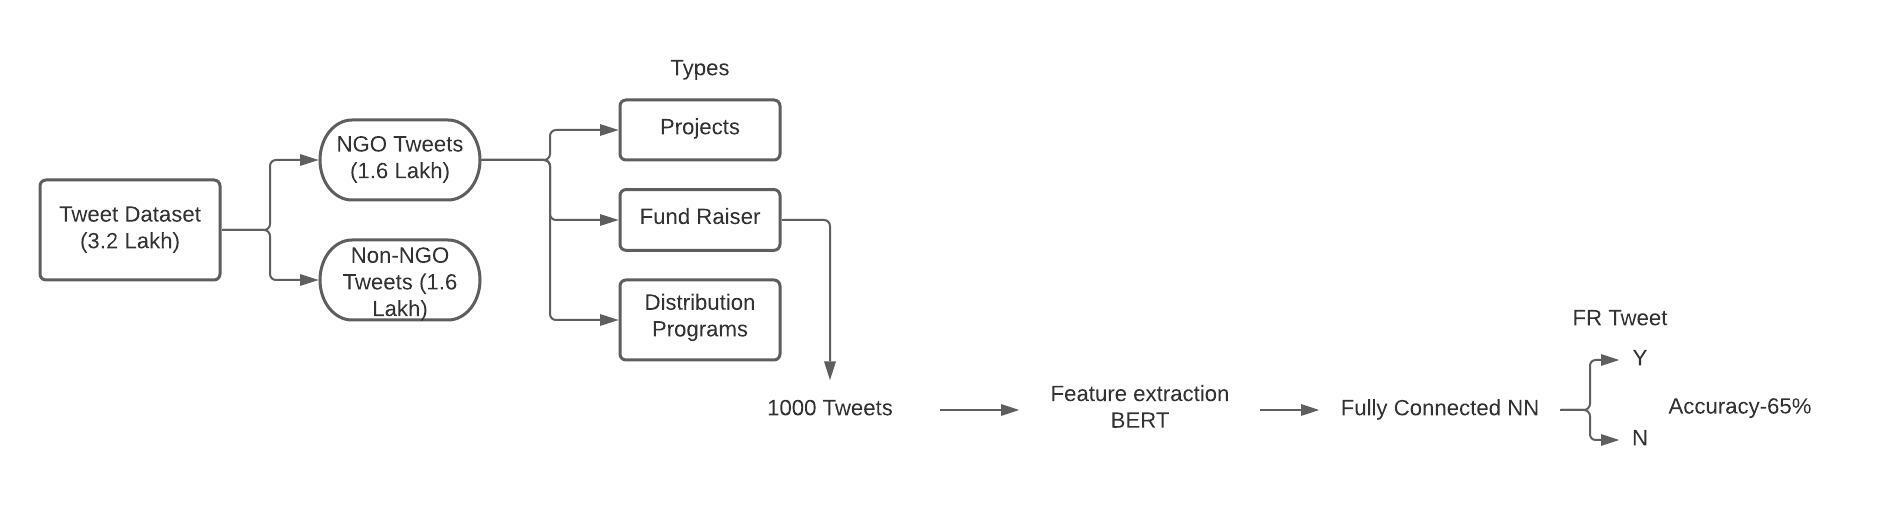
\includegraphics[scale=0.6]{Tweet Analysis.jpeg}
%     \caption{Flowchart for Model 2 without Augmentation}
% \end{figure*}

% \begin{figure*}
%     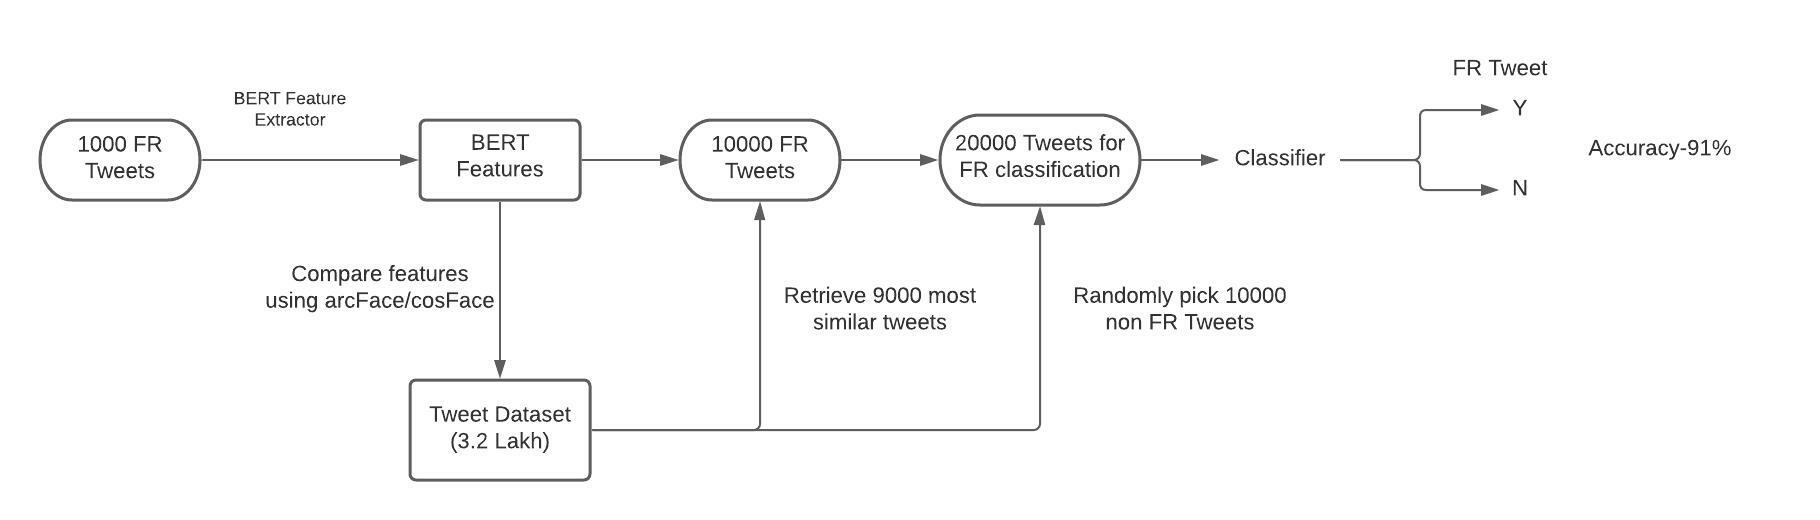
\includegraphics[scale=0.6]{Tweet Analysis 2.jpeg}
%     \caption{Flowchart for Model 2 with Augmentation}
% \end{figure*}

\begin{figure*}
    \centering
    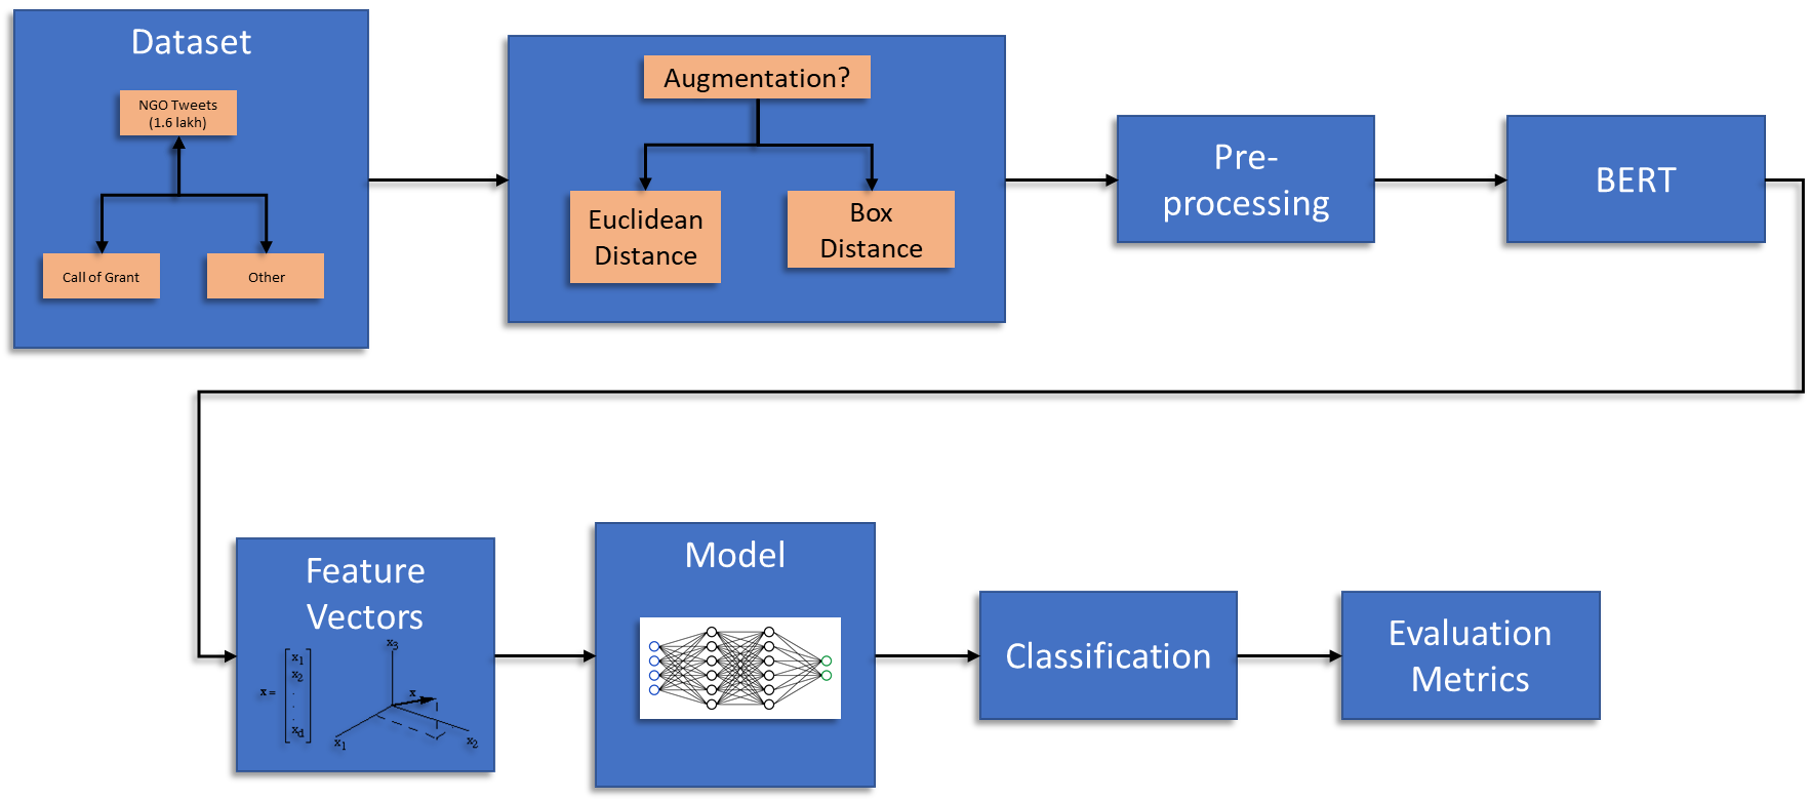
\includegraphics[scale=0.4]{Picture1.png}
    \caption{Model Flowchart}
    \label{fig:my_label}
\end{figure*}


\section{Related Works}
The HTC is a sub-problem of multi-label text classification. There are two extreme approaches to the problem --- local and global. The local models focus on classifying locally (or level wise) and later exploit the inherent hierarchy in a top-down fashion to restructure the output. On the other hand, the global models consider the entire hierarchy at once to classify for each level.

Another classification of the models is as static and dynamic models. For static models, the hierarchy is fixed and a characteristic of the pipeline, whereas in dynamic models, the hierarchy is not explicitly programmed in the pipeline. As we aim to design a pluggable model, it must be local and static by design.

To design our pipeline, we apply transfer learning as in \cite{pmlr-v80-wehrmann18a} and not multi-task learning as in \cite{shimura-etal-2018-hft} and \cite{banerjee-etal-2019-hierarchical}, particularly because the latter leads to a non-pluggable design. The design proposed in the next section is inspired by the HMCN-F architecture presented in \cite{pmlr-v80-wehrmann18a} --- a feedforward design of Multi-Layer Perceptron (MLP) blocks with cascade connections. However, to make the model pluggable, we eliminate the cascade forward connections for the baseline. The main drawback of static and local approaches is the large size of the pipeline and hence the number of parameters.

An improvement on HMCN-F and HMCN-R in \cite{pmlr-v80-wehrmann18a} is proposed in LA-HCN \cite{zhang2021lahcn}, which employs a label-based attention mechanism to better capture the inter-dependencies.

\section{Methodology}
Here we have discussed the dataset prepared and the baseline model's design. Our task has a two-level hierarchy: Non-Profit ($L_1$), Call of Grant ($L_2$). We first train the model for $L_1$, and we found a two-layer MLP to be sufficiently efficient for the same. For $L_2$, we had a limited set of examples and therefore observed menial performance, and to counter the same, we propose our neighborhood exploration strategy for augmenting text data in a later section.
\subsection{Dataset}
Due to the lack of available datasets pertaining to our use-case, we have generated a dataset from scratch. For the same, we were given a set of Twitter Handles belonging to organisations and persons who routinely tweet about our domains of interest. Using the Twitter API\footnote[1]{Reference: \url{https://developer.twitter.com/en/docs/twitter-api}}, we iteratively fetch tweets from the Twitter Handles.
Our ideal dataset, $D$, is structured as a binary tree of height two, its levels being denoted by $L_1$ and $L_2$.
\begin{equation}
    \forall L_{i+1} \text{  where  } i = 1, 2, L_i \subset L_{i}.
\end{equation}


\begin{figure} 
    \centering
    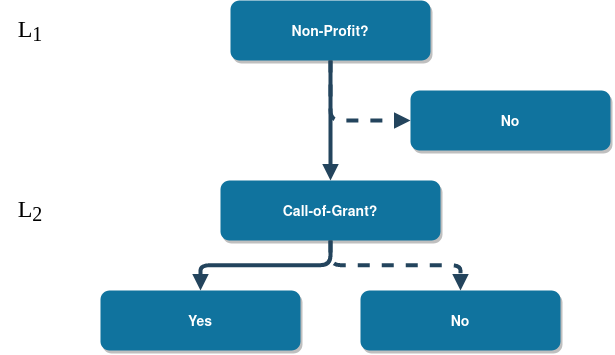
\includegraphics[width=0.80\linewidth]{Dataset.png}
    \caption{Dataset Representation}
\end{figure}


The initial set of tweets for the construction of context/$L_1$ contain a total of $179,845$ tweets collected from $1,967$ Twitter handles. After further preprocessing, we had a total of $165,456$ tweets. Out of which $1,050$ tweets were for $L_2$, we explore ways to expand the dataset in the next section. This data was used to first train a classification head for $L_1$ --- a single dense layer of dimension $(768, 1)$ which classifies the tweets based on the \textit{[CLS]} token's embedding. The testing set contains $650$ labelled examples.

The dataset has been augmented using two techniques: Euclidean and Box distance. For Euclidean distance, we select the closest 10 neighbours and all the points within a radius of 2 units. As for Box distance, we select all the points within a radius of 50 units.


\subsection{Pipeline}
A design approach for our relatively small set of classes could be to ignore the inductive bias of hierarchy among the classes entirely and obtain the classification probabilities on per class basis and later use them to restructure it into a hierarchy. This approach could potentially save model parameters, but instead, we choose to retain the inductive bias as it is integral to ensure modularity. One more reason to design a static model is to consider that at any point if the model specifies the tweet $T$ as $T \notin L_i$ \text{ then } $T \notin L_{j}$ $\forall j > i$ from (1). In addition, as our application is real-time, it must be as robust as possible. Thus, propagating through the unnecessary hidden-states is a huge overhead. To counter this, a static model can let us use the last accepted level's output directly.

Our hypothesis is based on Transfer Learning (TL). As the TL is by design reusing the model parameters, we conclude that our model should inherently apply TL at different stages of the classification. Further, we break the model into pluggable modules, following the encoder-decoder design paradigm. To do this, we replace the level-specific classification head with an adapter and a decoder for the next level. In the baseline, we use MLPs for the encoders, decoders, and adapters.
Given the informal nature of text on Twitter, language encoders such as the original BERT \cite{devlin2019bert} which have been trained on formal texts such as Wikipedia may not be effective. Another issue could be that the number of characters in tweets is capped at $280$, which in general makes them smaller than a typical Wikipedia paragraph. Therefore the LE might lose context when working with such small texts. To tackle this, we apply BERTweet \cite{bertweet}, which has been pre-trained on $850$ million English tweets, around $16$ billion word tokens and $80$ GiBs of data. Its performance is state-of-the-art for Twitter-related text inference/NLP tasks, and therefore, it generates appropriate dense word embeddings for our task.
% \begin{figure}[H]
%     \centering
%     \begin{subfigure}[b]{0.5\textwidth}
%             \centering
%             \includegraphics[width=\linewidth]{assets/$L_1$.png}
%             \caption{Level 1 (Non-Profit)}
%     \end{subfigure}\\
%     \begin{subfigure}[b]{0.75\textwidth}
%             \centering
%             \includegraphics[width=\linewidth]{assets/L2.png}
%             \caption{Level 2 (Call of Grant)}
%     \end{subfigure}\\
%     \begin{subfigure}[b]{\textwidth}
%             \centering
%             \includegraphics[width=\linewidth]{assets/L3.png}
%             \caption{Level 3 (Health-Education)}
%     \end{subfigure}
%     \caption{Preliminary Design}
%     \label{fig:design}
% \end{figure}\\\\
The following equations give a layer-wise flow of data during the inference/training.
\begin{equation}
    L_{1D} = L_{1E}(\text{BERT})
\end{equation}
\begin{equation}
    L_{2D} = L_{2 E}(L_{1,j A}(L_{1 E}))
\end{equation}
The adapter layers ($L_{j-1,j A}$) are an interface when extending the model for the next level and are intended to compensate for the down-scaling of the encoder output in the pre-training.

While training for level $j$, we froze all layers before $L_{j-1,j A}$. This way, we could have a modular model that extends the previous level's knowledge $L_{j-1}$ through Transfer Learning for the current level $L_j$.

\subsection{Model 1: Non-Profit Data vs NOT}
Here we create a model to classify tweets as Non-Profit or Not Non-profit. Non-profit data is taken as positive examples and Not non-profit data is taken as negative examples. The train-test split is 70\% and 30\% that is picked randomly. The model diagram is shown in Fig. 1. The tweets are given as input to BerTweet that gives a 786D vector as output. Following this, 2 FCNN layers are introduced that classifies the tweets. 99\% accuracy is achieved.

\subsection{Model 2}
Out of a corpus of 3.2 lakh tweets, given 1000 tweets labelled as fundraiser, the objective is to classify tweets into fundraiser and non-fundraiser categories. The training data used are these 1000 tweets. The model diagram can bee seen in Fig. 2. The model consists of a BERT feature extractor that will take the tweets as input and give feature vectors of size 768 as output. These feature vectors are then passed into a fully connected neural network that has its final layers modified into a classifier. This will consist of the entire model pipeline. The model will be trained end-to-end on multiple epochs and \emph{is expected to give an accuracy of about 65\%.}\\

\emph{Next Steps:}
To increase the labelled training data, methods such as arcFace and cosFace are used. Using these techniques, we can get more data from the 3.2 lakh tweets that can be labelled as fundraiser. The dataset will now consist of about 10,000 tweets labelled as fundraiser and an additional 10,000 tweets labelled as non-fundraiser. We will then re-train the classifier from step 1 using this larger dataset.



\section{Experiments}

For Model2, we tried 3 variants of BERT as given in the table below with FC(256, 512) on data containing cogData and 1000 random tweets from the Not for Profit data. The data was spilt into 70\% for train and 30\% for validation and trained for 50 epochs.

\begin{table*}[t]
\centering
\resizebox{\textwidth}{!}{\begin{tabular}{|c|c|c|c|c|c|c|}
 \hline
 & \multicolumn{2}{|c|}{\textbf{Without Augmentation}} & \multicolumn{2}{|c|}{\textbf{Augmentation Using Euclidean}} & \multicolumn{2}{|c|}{\textbf{Augmentation Using Box Distance}}  \\
 \hline
 
 \textbf{Model} & Accuracy & F1 & Accuracy & F1 & Accuracy & F1 \\
 \hline
 
 Neural Network & 0.965 & 0.954 & 0.81 (Top 10), 0.94 (Radius=2) & 0.81 (Top 10), 0.941 (Radius=2) & 0.94 (Radius=50) & 0.934 (Radius=50) \\
 \hline
 
 Naive Bayes & 0.926 & 0.9253 & 0.816 (Radius=2) & 0.821 & 0.783 & 0.756  \\
 \hline
 
 SVM & 0.953 & 0.939 & 0.831 (Radius=2) & 0.836 & 0.838 & 0.832  \\
 \hline
%  cogData+1000 NP tweets from original dataset & 95.65\%  \\
% \hline
% cogData+1000 NP tweets after removing duplicate tweets from original dataset  & 94.1\%  \\
% \hline

\end{tabular}}
\caption{Experiments}
\label{Table 1}
\end{table*}


\begin{tabularx}{0.4\textwidth} { 
  | >{\raggedright\arraybackslash}X 
  | >{\centering\arraybackslash}X 
  | >{\raggedleft\arraybackslash}X | }
 \hline
 \textbf{BERT Model} & \textbf{Accuracy}  \\
 \hline
 bert-base-nli-mean  & 98\%  \\
\hline
bert-base-uncased  & 92\%  \\
\hline
BerTweet  & 97\%  \\
\hline

\end{tabularx}

\textbf{RobertaForSequenceClassification} was considered next for the experiments with BerTweet as the BERT tokenizer. The model was trained on similar data split as mentioned above for 30 epochs. Four experiments were performed on the above mentioned model. For Euclidean Distance, two cases were experimented with: taking top 10 nearest points for each Cog data point and taking all data points less than 2 units away for each Cog datapoint. We also perform three experiments each on the same data using \textbf{Naive Bayes} and \textbf{SVM}. The results of the experiments are mentioned in Table 1.

% \begin{tabularx}{0.4\textwidth} { 
%   | >{\raggedright\arraybackslash}X 
%   | >{\centering\arraybackslash}X 
%   | >{\raggedleft\arraybackslash}X | }
%  \hline
%  \textbf{Experiment} & \textbf{Accuracy}  \\
%  \hline
%  cogData+1000 NP tweets from original dataset & 95.65\%  \\
% \hline
% cogData+1000 NP tweets after removing duplicate tweets from original dataset  & 94.1\%  \\
% \hline

% \end{tabularx}



\printbibliography


\end{document}
